\documentclass{trnotes}
\setlayout{hardcopy}
\geometry{left=2cm, right=2cm}
\usepackage{trmath}
\usepackage{trsym}
\setmainfont{PT Serif}[
  BoldFont = {Lato Semibold}
]
\setsansfont{Lato}
% \setmonofont{CMU Typewriter Text}
\setmathfont{STIX Two Math}
% Use XITS Math for    [     ]     (     )     {     }
% \setmathfont[range={"005B,"005D,"0028,"0029,"007B,"007D}]{XITS Math}
\setmathfont[range={"007B,"007D}]{XITS Math}
\renewcommand{\baselinestretch}{1.5}

\title{\vspace{-1em}<<Антарес>>: вступительный тест}
\date{\vspace{-2em}30 сентября 2020 г.}
\begin{document}
\maketitle

\begin{center}
  \fboxsep=2ex
  \fbox{\parbox{5.5in}{\centering
    Ответы на вопросы напишите на этом же листе.\\
    Пугаться не нужно, это не контрольная и оценок никто ставить не будет :)
  }}
\end{center}

\section*{Расскажите о себе}
\makebox[\textwidth]{ФИО и класс:\enspace\hrulefill}
\makebox[\textwidth]{Как связаться (почта, телефон, соцсети):\enspace\hrulefill}


\vspace{1em}

\section*{Вопросы}

\begin{enumerate}
  \item Отметьте изображение спутника планеты Солнечной системы.

    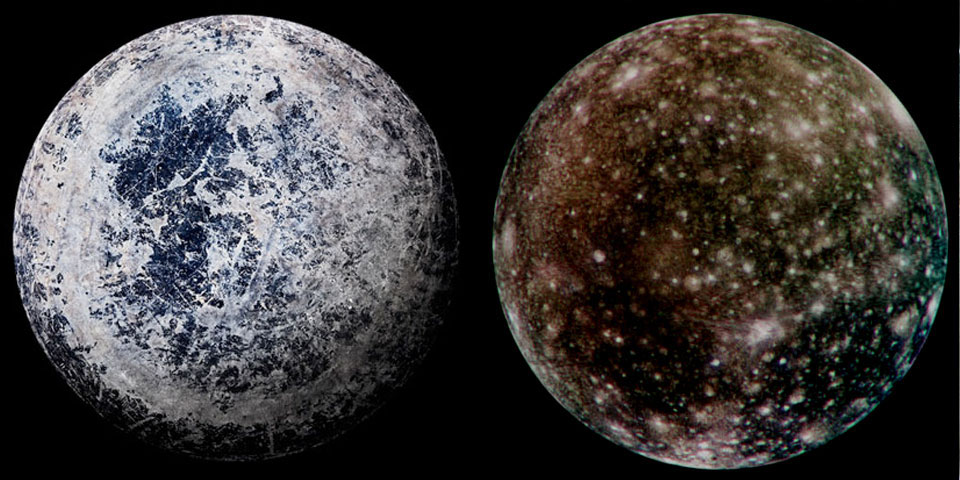
\includegraphics[width=0.9\textwidth]{im1.png}\\
    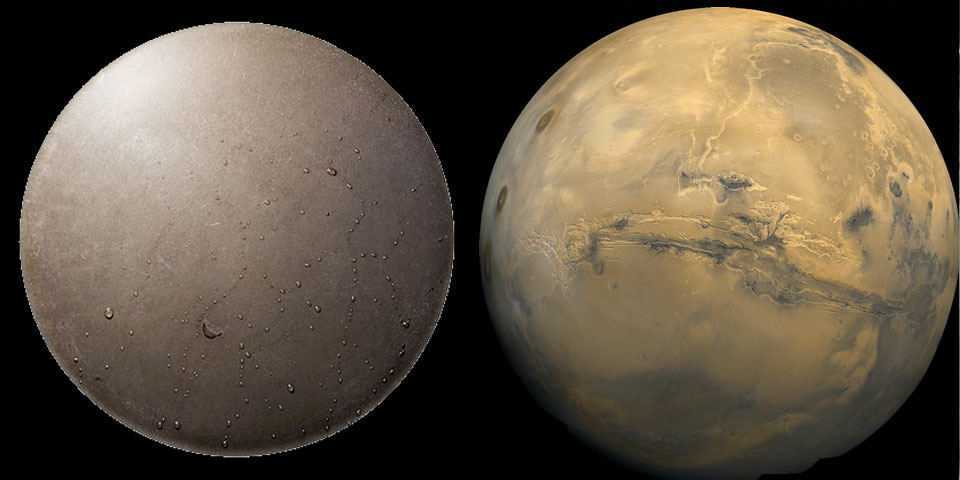
\includegraphics[width=0.9\textwidth]{im2.png}
  \item Какая из фраз наиболее точно отражает положение Солнца в нашей Галактике?
    \begin{enumerate}[a)]
      \itemsep=0pt \parsep=0pt
      \item Солнце находится в центре Вселенной
      \item Солнце находится в галактическом балдже 
      \item Солнце находится вне диска галактики
      \item ``Наша хата с краю''
    \end{enumerate}
  \item Вам предлагают два бинокля: один с тридцатикратным увеличением, но в диаметром объектива 50см, другой 20кратный, но 80см. Какой лучше подходит для астрономических наблюдений и почему? Можете предположить, что фокусные расстояния окуляров --- одинаковые.
    \begin{enumerate}[a)]
      \itemsep=0pt\parsep=0pt
      \item Первый, у него больше светосила.
      \item Второй, у него больше светосила.
      \item Тот, у которого больше увеличение.
      \item Оба не подходят.
    \end{enumerate}
  \item 10 декабря 2018 года космический аппарат «Вояджер-2» преодолел гелиопаузу. К этому времени сигналы с него приходили с задержкой 16.5 часов. Оцените, на каком расстоянии от Солнца находится гелиопауза?
    
    \vspace*{7em}

\makebox[\textwidth]{Ответ:\enspace\hrulefill}
  \item Если бы в полночь 27го сентября 2020 года в окрестности Санкт-Петербурга Вы посмотрели в юго-восточную часть горизонта, перед Вашим взором (а ночь была ясная) бы предстало яркое небесное тело красноватого оттенка. Что это?
    \begin{enumerate}[a)]
      \itemsep=0pt\parsep=0pt
      \item Юпитер
      \item Альдебаран
      \item Нибиру летит!
      \item Марс
    \end{enumerate}
  \item В некоторой точке Земли звезды Дубге и Мерак ($α$ и $β$ Большой Медведицы) одновременно появились над горизонтом. Где мог находиться наблюдатель? 
    \begin{enumerate}[a)]
      \itemsep=0pt\parsep=0pt
      \item На экваторе
      \item На северном полюсе
      \item На $60^\circ$ cеверной широты.
      \item Это невозможно
    \end{enumerate}

\end{enumerate}
\end{document}
